%
\section{Image Tree Based on Wordnet}
\label{sec_wordnetsearchtree}

\subsection{Wordnet}\index{Wordnet}
The offical web page \footnote{http://wordnet.princeton.edu/} describes WordNet as a freely and publicly available "large lexical database of english nouns, verbs, adjectives and adverbs, grouped into sets of cognitive synonyms (\emph{Synsets}\index{Synset}), each expressing a distinct concept." That is, a Synset is a particular concept which can be expressed by different terms but has one unique identifier. The identifier consists of the word most commonly used to describe the concept, the part of speech, and a number, e.g. \emph{drive.v.02}.\\
The number is necessary because one word can have multiple meanings that will then be represented by different synsets, like in \emph{cherry.n.01} for the tree and \emph{cherry.n.02} for the fruit. \\

Synsets are linked with each other through several semantic relations, e.g. hyponyms or meronyms.
In our work, we use this network of synsets to discover the semantics between terms describing the images as well as towards the search term. \\
  
  
\subsection{Synset Detection}
The first step now is to identify valuable image annotations and associate them with their meaning, i.e. find the Synset they represent. \\
We considered the following annoations provided by the Flickr API and evaluated them on twenty randomly sampled pictures: 
\begin{itemize} 
\item{\emph{Title.}} The title was usually a short but precise description of the image content and thus very valuable for semantic annotation.
\item{\emph{Description.}} The description did often relate to the image content but with a lot of fill words and noise as well as context-dependent meanings, so it could be useful but would require additional preprocessing such as Named Entity Recognition.
\item{\emph{Comments.}} Only very few comments described the image in any way - they were mostly used for social interaction with the photographer. 
\item{\emph{Tags.}} \todo{describe what we found out about tags, groups, and albums and why we (do not) use them}
\item{\emph{Group Names.}}  preprocessing needed to match any to wordnet
\item{\emph{Album Names.}}  preprocessing needed to match any to wordnet
\end{itemize}

Based on these findings, we use the separate words from the title as well as tags, and try to find the corresponding Synset. We limit this matching to nouns, for two reasons: First, nouns are usually the words describing the depicted concepts. Second, the method described below to find the best matching Synset does not work across different parts of speech. \\

The difficulty with the Synset\index{Synset} detection is that there are multiple possible Synsets for a word, and it is obvious to a human observer but not to a computer which meaning is correct. Assuming that annotations on each image are closely related because they describe the same image content, we use those Synsets that, altogether, give the smallest semantic distance across all annotations of an image. Semantic distance of two terms can be measured by the length of the path between them in the WordNet tree. We use the Leacock and Chodorow Normalized Path Length (LCH-Similarity) provided by WordNet, which uses adapted weights and normalization factors, because it is perceived as closer to human understanding than regular path similarity \cite{budanitsky01}.\\

To efficiently find the set of Synsets with the smallest overall distance, a best-first search algorithm \footnote{Please refer to Artificial Intelligence literature for a detailed explanation.} is used. Note that such search algorithms require non-negative distances between options, but WordNet provides similarities. To convert them into distances without changing the scale, the similarity is simply subtracted from the maximally possible similarity, i.e. the similarity of a Synset to itself, which is roughly 3.7.
For complexity reasons, only the best 100 candidates are considered at any time. Of course, this does not guarantee the perfect result anymore, but other paths are highly unlikely to become the best candidate in the end, and keeping all candidates would decrease performance significantly. \\
still erroneous with words that are meant in a way that is unknown to WordNet, i.e. canon as the camera model is interpreted as [definition of canon.n.01]  \\
therefore preprocessing removes all tags that include numbers. Blacklist could filter even more but would also filter canon in its real sense, and generally not desirable to be flexible with respect to the tag vocabulary.  \\
also removes special characters (more likely to be found on WordNet, and more likely to be identical with other unmatchable tags) 


\subsection{Constructing a Searchtree} 
In general, all words represented in WordNet can be used as a query term for our tool. For the given use case, however, queries will be limited to those that can be seen in pictures. This is mainly the case for object descriptors at various levels of specificity, and place names, so our work is focused on these types of search terms.

When a term is entered into the tool, it is first used to retrieve all Synsets\index{Synset} that can be expressed by this term.
actually construct multiple searchtrees if more than one synset found for a searchterm (i.e. train coach and motorized vehicle for car)\\
use hyponym relation to span tree of specializations (i.e. apple, banana for fruit; bus, sportscar for car)\\
if no hyponyms (usually the case for geographic terms), use part-meronyms\\

\begin{figure}
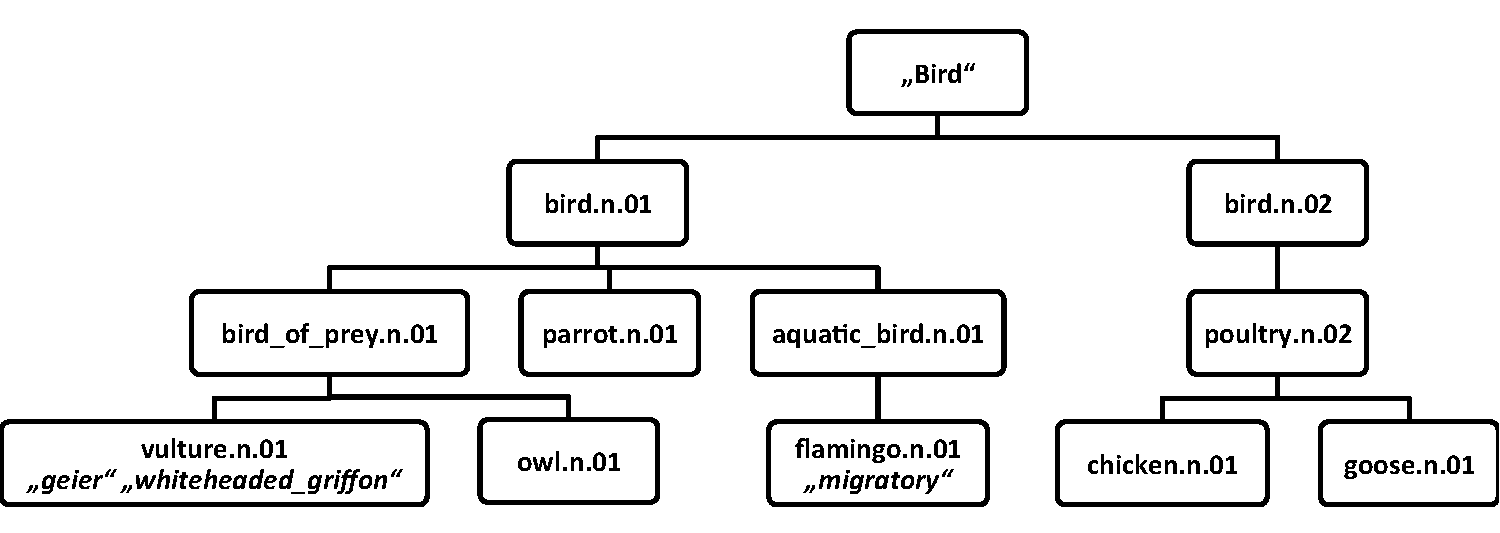
\includegraphics[width=\textwidth]{images/searchtree.pdf}
\caption{todo}
\label{fig_searchtree}
\end{figure}


\subsection{Assigning Pictures to Tree Nodes}
for higher recall: find strongly co-occurring tags that could not be mapped to synset \\
strong co-occurrence defined on tf-idf (else camera models would be strong co-occurrence with many synsets)
observed that it is useful to find translations etc. but of course also introduces noise; choice of threshold (currently $0.75 * max_tf_idf$, where max tfidf is the maximal score across all values) \\
take all pictures that are annotated with at least one of the related tags or the synset itself. parameter \emph{minimal node size}: if not fulfilled, node is integrated into parent node (union pictures into parent's pictures)
